\documentclass[a4paper,10pt]{article}
\usepackage[MeX]{polski}
\usepackage[utf8]{inputenc}
\usepackage[pdftex]{graphicx}
\usepackage{fancyhdr}
\usepackage{lastpage}
%\author{}
\title{Gazeta}
\pagestyle{fancy}
\fancyhead{}
\lfoot{\scriptsize Plik: gazeta.pdf\\Copyright \copyright\ Akademia Górniczo-Hutnicza}
\cfoot{\scriptsize Wersja: \textbf{0.1} z dnia 26.12.2007 
\\\normalsize \thepage}
\rfoot{\scriptsize Stron: \pageref{LastPage} Długość: ? kB\\Prowadzenie zajęć:}
\renewcommand{\headrulewidth}{0pt}
\renewcommand{\footrulewidth}{0.5pt}
\usepackage[pdftex]{hyperref} %ma być ostatnie w~preambule

\begin{document}
%strona tytułowa
\begin{center}
\mbox{\Huge AKADEMIA GÓRNICZO\dywiz HUTNICZA}\\
\mbox{\Large Wydział Elektrotechniki, Automatyki, Informatyki i~Elektroniki}\\

\includegraphics[scale=0.5]{gfx/agh.jpg}\\
\mbox{\Large KATEDRA INFORMATYKI}
\end{center}
%TODO tabelka na dole pierwszej strony
%TODO marginesy pierwszej strony (żeby nagłówek się mieścił i~był równo)
\thispagestyle{empty}
\clearpage

%copyright i~spis treści
\begin{tabular}{|p{12cm}|}
\hline
Niniejsze opracowanie powstało w~trakcie i~jako rezultat zajęć dydaktycznych z~przedmiotu wymienionego na stronie tytułowej, prowadzonych w~Akademii Górniczo\dywiz Hutniczej w~Krakowie (AGH) przez osobę (osoby) wymienioną (wymienione) po słowach ``Prowadzący zajęcia'' i~nie może być wykorzystywane w~jakikolwiek sposób i~do jakichkolwiek celów, w~całości lub części, w~szczególności publikowanie w~jakikolwiek sposób i~w~jakiejkolwiek formie, bez uzyskania uprzedniej, pisemnej zgody tej osoby (tych osób) lub odpowiednich władz AGH.\\
\\
\textbf{Copyright \copyright\ Akademia Górniczo\dywiz Hutnicza (AGH) w~Krakowie}\\
\hline
\end{tabular}
\tableofcontents
\clearpage

%treść
\section{Koncepcja}
\subsection{Zleceniodawca}
Nasz projekt będzie realizowany na zlecenie firmy North Press, która zajmuje się
prowadzeniem sieci salonów prasowych Świat Prasy. Potrzebuje ona systemu umożliwiającego
sprawne monitorowanie sprzedaży i~stanu magazynów, ułatwiającego podejmowanie decyzji w~kwestiach
logistyki, a~także wspomagającego generowanie zamówień do dostawców, faktur dla
klientów oraz dziennych raportów ze sprzedaży.

\subsection{Ogólna wizja projektu}
System, który zaprojektujemy, ma za zadanie zbierać dane dotyczące sprzedaży ze wszystkich
stanowisk kasowych (używane w~tej chwili kasy fiskalne umożliwiają przesyłanie danych pomiędzy
kasą, a podłączonym do niej komputerem) i~umożliwiać ich analizę kierownictwu firmy, a~także
samym kasjerom, jak również ułatwiać im podejmowanie decyzji dotyczących zamawiania i~składowania
towaru\footnote{Dość niefortunne określenie dla książek i~czasopism, ale bierzemy pod uwagę,
że w~salonach sprzedawane są także papierosy, gumy do żucia, kupony pre-paid, bilety MPK, etc.}
na podstawie uzyskanych danych.

Podstawowe funkcje, które system powinien spełniać, to:
\begin{itemize}
    \item zbieranie i~przechowywanie danych dotyczących sprzedaży mających miejsce we wszystkich salonach
    \item zbieranie i~przechowywanie danych dotyczących towaru składowanego we wszystkich salonach,
    z~możliwością wglądu również dla kasjerów (w celu ułatwienia im sprawdzenia, czy dany towar jest
    możliwy do nabycia w~tym lub innym salonie, a~także w~jakiej ilości jest tam przechowywany)
    \item generowanie raportów sprzedaży
    \item generowanie faktur dla klientów oraz księgowanie faktur wystawionych przez dostawców.
    \item analiza wydajności poszczególnych pracowników i~salonów (również z~uwzględnieniem określonych przedziałów czasowych)
    \item analiza popytu na poszczególne towary w~salonach
    \item sugerowanie (po analizie popytu i~sprzedaży) wysokości zamówień do dostawców na poszczególne towary oraz generowanie tychże
    \item sugerowanie (po analizie popytu) miejsca i~proporcji przechowywania poszczególnych
    towarów (np.\ 200 sztuk ,,Przyjaciółki'' w~salonie nr 1, 150 sztuk w salonie nr 2, 40 w salonie
    nr 3), z~uwzględnieniem możliwości przechowywania w~każdym z~miejsc branych pod uwagę
    \item sugerowanie (po analizie sprzedaży i~stanu poszczególnych magazynowego w~salonach w~chwili bieżącej)
    przetransportowania określonej ilości towaru do danego salonu, aby zdołał on zaspokoić popyt
    \item sugerowanie (po analizie wydajności) wprowadzenia zmian w~godzinach otwarcia poszczególnych salonów
\end{itemize}

Rozważamy też rozszerzenie projektu o~dodatkowe funkcje, jak na przykład system punktowy dla
stałych klientów lub możliwość prenumeraty czasopism i~wydawnictw cyklicznych (z~możliwością
wysyłki pocztą/kurierem lub odbioru osobistego). Decyzja na ten temat zostanie podjęta po
rozmowach z~zleceniodawcą.


\section{Zakres odpowiedzialności systemu}
\begin{enumerate}
\item Zarządzanie listą towarów sprzedawanych przez sieć.
\item Zarządzanie ofertą każdego z~salonów na podstawie listy towarów.
\item Zbieranie informacji nt.\ sprzedaży danego towaru w~przeszłości.
\item Zarządzanie stanem magazynowym każdego z~saloników.
\item Generowanie i~przekazywanie dokumentów używanych w~przedsiębiorstwie (dokumenty magazynowe, faktury od dostawców).
\item Wystawienie faktury kupującemu.
\item Generowanie statystyk dotyczących aktywności saloników w~określonych porach dnia i~dniach tygodnia.
\item Generowanie statystyk dotyczących sprzedaży poszczególnych towarów globalnie oraz w~poszczególnych salonach.
\item Komunikacja pomiędzy salonikami, a~osobą zarządzającą w~zakresie bieżących zmian cen oraz kodów PLU towarów.
\item Generowanie dzienników utargów kasowych (rozliczeń zmiany).
\item Wprowadzenie odpowiednich ustawień do kasy fiskalnej na podstawie informacji o~ofercie danego salonu.
\end{enumerate}


\section{Dziedzina problemu}
Opracowywany system informatyczny przeznaczony jest dla sieci salonów prasowych Świat Prasy będących własnością firmy North Press. W~chwili obecnej (listopad 2007) sieć obejmuje województwa Kujawsko-Pomorskie, Pomorskie oraz Warmińsko-Mazurskie. System będzie używany przez pracowników zarządzających przedsiębiorstwem oraz obsługę salonów (w~szczególności kierowników salonu). Towar dostarczany jest bezpośrednio do salonu, a~jego obsługa zobowiązana jest do dokonania w~systemie odpowiednich czynności związanych z~tą dostawą.

Pracowników przedsiębiorstwa można podzielić na trzy główne grupy: zarządzający, kierownicy saloników, pracownicy saloników.

Zadaniem zarządzających jest obsługa (wprowadzanie, usuwanie, zmiana) informacji dotyczących towarów sprzedawanych w~salonikach, w~szczególności ustalanie ceny, stawek podatku, kodów kreskowych PLU (ang.\ \emph{Price Look-Up}) oraz przynależność towarów do odpowiedniej grupy towarów; zarządzanie ofertami konkretnych saloników, w~tym ustalanie rzeczywistej ceny sprzedaży w danym salonie, upustów, rabatów oraz określenie dostawcy danego towaru do danego saloniku. Zarządzający mają wgląd do dokumentów generowanych przez salony, lecz nie modyfikują ich. Ponadto zarządzający otrzymują informacje na temat sprzedaży i~obrotów w~każdym z~saloników.

Pracownicy salonów mają możliwość zmienić ustaloną przez zarząd cenę danego towaru (np.\ gazeta przychodzi od dostawcy z~nadrukowaną inną ceną niż miała dotychczas), lecz o~tej zmianie zobowiązani są poinformować zarządzającego. Zarządzający potwierdzą tę zmianę lub odrzuca. W przypadku potwierdzenia może również podjąć decyzje o~zmianie ceny w~pozostałych salonach. Pracownicy salonów mogą zmieniać też kody PLU zapisane w~kasie (np.\ z~powodu zmiany kodu artykułu) o~czym również informują zarządzającego. Pracownik przyjmujący dostawę towaru zobowiązany jest udokumentować ją tworząc dokument przyjęcia do magazynu. Dokument ten dostępny jest do wglądu dla kierownika salonu oraz dla zarządu. Generowane są także dokumenty wydania z~magazynu (np.\ w~przypadku zwrotów prasy do dostawcy). Jeżeli dostawca razem z~dostawą pozostawia w~salonie fakturę, faktura ta musi być przez pracownika salonu przekazana osobie zarządzającej. Po zakończeniu zmiany w~salonie dokonywane jest rozliczenie tej zmiany zawierające informacje na temat stanu kasy na zakończenie (ilość banknotów każdego rodzaju, wartość bilonu, ilość i~wartość płatności kartą, wartość zasiłku zostawionego na kolejną zmianę). Ponadto kierownik salonu dysponuje analogicznymi informacjami na temat sprzedaży i~obrotów jak zarząd, jednakże dotyczącymi wyłącznie jego salonu.

Ponadto od czasu do czasu pracownicy zarządzający wykonują również zadania przeznaczone z założenia dla pracowników salonu.

Każdy z~salonów działa niezależnie od pozostałych, tzn.\ zwykle nie przenosi się towaru, ani środków finansowych pomiędzy nimi, aczkolwiek czasami dokonuje się operacji przeniesienia towaru. Wówczas tworzone są dokumenty wydania i~przyjęcia do magazynu.

Każdy z~salonów dysponuje połączeniem z~internetem (ADSL lub GPRS) oraz kasą fiskalną \textbf{JAKA KASA???} wraz z~czytnikiem kodów kreskowych.
%TODO wybrać kasę


\section{Baza danych}
\begin{figure}
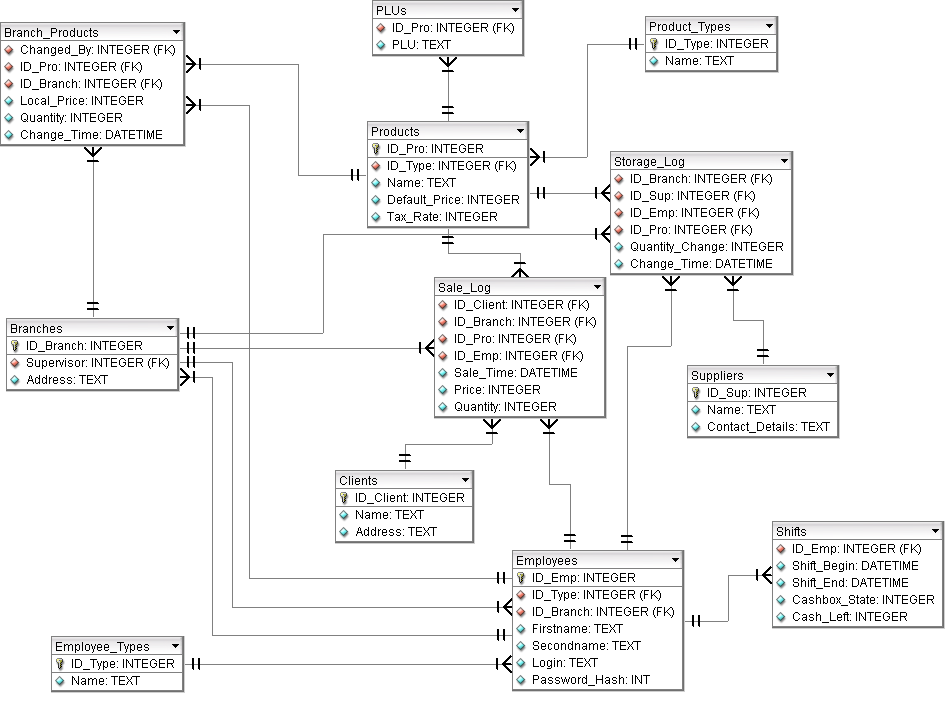
\includegraphics[width=1\textwidth]{gfx/baza.png}
\caption{Schemat bazy danych}
\end{figure}
Opis tabel:
\begin{description}
\item[Branches] każdy rekord tabeli odpowiada jednemu salonowi
    \begin{description}
    \item[ID\_Branch] - identyfikator salonu (klucz główny)
    \item[Supervisor] - identyfikator kierownika salonu (klucz obcy do tabeli Employees)
    \item[Address] - adres salonu
    \end{description}
\item[Employees] dane pracowników
    \begin{description}
    \item[ID\_Emp] - identyfikator pracownika (klucz główny)
    \item[ID\_Branch] - identyfikator salonu, w którym pracuje dany pracownik (klucz obcy do tabeli Branches)
    \item[Firstname] - imię pracownika
    \item[Secondname] - nazwisko pracownika
    \item[Login] - nazwa pracownika w systemie
    \item[Password\_Hash] - skrót kryptograficzny hasła pracownika
    \end{description}
\item[Shifts] zmiany pracowników
    \begin{description}
    \item[ID\_Emp] - pracownik, którego dotyczy dana informacja o zmianie (klucz obcy do tabeli Employees)
    \item[Shift\_Begin] - czas rozpoczęcia zmiany
    \item[Shift\_End] - czas zakończenia zmiany
    \item[Cashbox\_State] - stan kasy na zakończenie zmiany
    \item[Cash\_Left] - wartość zasiłku pozostawionego kolejnej zmianie
    \end{description}
\item[Products] dane dotyczące produktów
    \begin{description}
    \item[ID\_Pro] - identyfikator produktu (klucz główny)
    \item[ID\_Type] - typ produktu (klucz obcy do tabeli Product\_Types)
    \item[Name] - nazwa produktu
    \item[Default\_Price] - domyślna cena produktu
    \item[Tax\_Rate] - wartość podatku, jakim objęty jest produkt
    \end{description}
\item[Branch\_Products] dane dotyczące produktów, w konkretnych salonach
    \begin{description}
    \item[Changed\_By] - pracownik, wprowadzający zmianę (klucz obcy do tabeli Employees)
    \item[ID\_Pro] - identyfikator produktu (klucz obcy do tabeli Products)
    \item[ID\_Branch] - identyfikator salonu (klucz obcy do tabeli Branches)
    \item[Local\_Price] - cena produktu w salonie
    \item[Quantity] - ilość produktu dostępnego w salonie
    \end{description}
\item[Sale\_Log] dziennik sprzedaży
    \begin{description}
    \item[ID\_Client] - identyfikator klienta otrzymującego fakturę lub NULL, jeżeli faktura nie została wydana (klucz obcy do tabeli Clients)
    \item[ID\_Branch] - salon, w którym nastąpiła sprzedaż (klucz obcy do tabeli Branches)
    \item[ID\_Pro] - sprzedawany produkt (klucz obcy do tabeli Products)
    \item[ID\_Emp] - pracownik odpowiedzialny za sprzedaż (klucz obcy do tabeli Employees)
    \item[Sale\_Time] - czas sprzedaży
    \item[Price] - cena
    \item[Quantity] - ilość
    \end{description}
\item[Storage\_Log] dziennik operacji na magazynie
    \begin{description}
    \item[ID\_Branch] - salon, którego dotyczy operacja (klucz obcy do tabeli Branches)
    \item[ID\_Sup] - identyfikator dostawcy (klucz obcy do tabeli Suppliers)
    \item[ID\_Emp] - pracownik odpowiedzialny za operację (klucz obcy do tabeli Employees)
    \item[ID\_Pro] - produkt, którego dotyczy operacja (klucz obcy do tabeli Products)
    \item[Quantity\_Change] - zmiana ilości stanu magazynu, wartość dodatnia oznacza przyjęcie towaru, ujemna --- wydanie
    \item[Change\_Time] - czas wykonania operacji
    \end{description}
\item[Product\_Types] typy produktów
    \begin{description}
    \item[ID\_Type] - identyfikator typu (klucz główny)
    \item[Name] - nazwa typu
    \end{description}
\item[Suppliers] dane dostawców
    \begin{description}
    \item[ID\_Sup] - identyfikator dostawcy (klucz główny)
    \item[Name] - nazwa dostawcy
    \item[Contact\_Details] - szczegóły dotyczące kontaktu z dostawcą
    \end{description}
\item[Clients] dane klientów (do faktur)
    \begin{description}
    \item[ID\_Client] - identyfikator klienta (klucz główny)
    \item[Name] - nazwa klienta
    \item[Address] - adres klienta
    \end{description}
\item[PLUs] kody PLU produktów
    \begin{description}
    \item[ID\_Pro] - identyfikator produktu (klucz obcy do tabeli Products)
    \item[PLU] - kod PLU
    \end{description}
\end{description}



%spis ilustracji i~tabel
\clearpage
\listoffigures
\listoftables
\end{document}

